\chapter{Phonemized CHILDES: A Phonemic Multi-Lingual Corpus of Child-Directed Speech}

\rough{Single paragraph introduction to chapter}

\section{Introduction}
\label{sec:dataset-intro}

\begin{roughdraft}
1. We want to do language modelling with phonemes, but finding suitable datasets is a challenge, especially considering particular requirements that we may want. These requirements are:
\begin{itemize}
    \item \textbf{Phonemic:} First requirement is that the data is in a suitable phonemic format, such as IPA. This already rules out many of the standard open-sourced language modelling datasets, which are orthographic.
    \item \textbf{Large:} Language models are data-hungry and so need suitable data. Exactly how much is explored in Chapter 4.
    \item \textbf{Parallel:} In order to establish the feasibility of language modelling with phonemes, and especially to compare phonemic modelling to orthographic modelling (as is done in Chapter 4), we ideally want to have corpora with utterances written both orthographically and phonemically.
    \item \textbf{Multilingual}: In order to compare the properties of different languages (chapter 5) or establish whether proposed language acquisition mechanisms are universal (chapter 6) we need a datasets that includes as many languages as possible.
    \item \textbf{Speech:} For comparing properties of spoken language (Chapter 5) and acquisition experiments (due to nature of input children receive, Chapter 6) we require data from speech sources.
    \item \textbf{Child-directed speech}: For acquisition work, CDS makes sense from what we know about the quality etc (Chapter 6). 
\end{itemize}

2. These are often competing requirements. Few phonemic datasets that are also large enough for LLMs due to the availability of phonemic transcriptions. Multilingual datasets are also difficult due to how dominant English is in research, yet alone when we also require them to be multi-lingual. 

3. There are some datasets that meet some of the requirements:
\begin{itemize}
    \item \textbf{CHILDES:} CHILDES description. Meets many requirements, but not much phonemic data. 
    \item \textbf{AudioBNC:} Audio BNC description. Meets many requirements but not CDS and not multilingual. 
    \item \textbf{BabyLM Pre-training data}: Describe. Good for evaluating models. 
    \item \textbf{\ldots:} 
\end{itemize}

4. Table here showing which datasets match which requirements. Clearly none match all the requirements we want for the work in this thesis, a good solution is \textbf{automatic phonemization} to convert CHILDES and BabyLM Pre-training data.

5. In this chapter, I first present the creation of \corpusphonemizer to address this challenge. I then introduce \phonemizedchildes, a dataset created using this tool which meets all these requirements and is used in Chapter 5 and Chapter 6. Finally, I use the parallel nature of Audio BNC to address the limits of automatic phonemization by comparing human phonemic transcriptions to the automated transcriptions generated from the parallel orthographic sentences.
\end{roughdraft}

Language modelling is a core task in NLP that involves learning the structure of language by making predictions of individual language units given a context. There is considerable variation in how the task is approached, whether it be the granularity of the language unit being predicted (such as words, characters or subwords), the model being used (n-gram models, RNNs, transformers) and the objective being optimised (such as next-token prediction or masked language modelling). In all cases, a dataset is required from which the distributed statistics of the language can be extracted.

The choice of dataset is largely determined by the application of the language model being trained. Particular datasets are often chosen according to the domain of the language  


If the goal is to learn the structure of language used in a particular domain, the dataset should contain language from that domain. For example, the Switchboard Corpus contains transcriptions of telephone conversations and was collected to improve language modelling of speech. For instance, in the early days of language modelling with n-grams, the Brown Corpus was used as a benchmark, containing 1 million words across various genres, such as news, fiction, and academic writing.


In the early days of language modelling with n-grams, the Brown Corpus was used as a benchmark when the goal was to develop  




Language modeling is the task of predicting the next word or sequence of words in a sentence based on the context, enabling machines to generate, understand, and process human language.

\section{Background}
\label{sec:dataset-background}

\rough{Related background to this work. Introduction to IPA. Introduction to the Phoneme Stream representation (motivated by past work and existing evaluation datasets). Maybe introduce Phoible here.}

\section{Corpus Phonemizer}
\label{sec:dataset-corpus-phonemizer}

In order to address the challenges of automatically converting orthographic datasets to phonemic streams, I developed \corpusphonemizer,\footnote{\url{https://github.com/codebyzeb/Corpus-Phonemicizers}} a suite of tools and scripts for converting corpora into datasets using a consistent phoneme stream representation.

The primary tool in the suite is a command-line application \texttt{corpus\_phonemizer.py} which takes orthographic text as input and converts it to a unified phonemic representation in IPA. The tool supports many languages by leveraging backend transliteration tools which can be selected by the user, each of which provides a different set of language codes (see \cref{sec:dataset-transliteration-tool-backends}).

A crucial component of the tool is the use of \emph{folding dictionaries} to ensure that the set of phonemes produced by the backend transliteration tool for a particular language matches a standard phonemic inventory for that language. This validation step is important, \todo{expand on this}. It is also important to ensure that when designing the folding dictionaries, a consistent methodology is used. In order to support my multi-lingual experiments, I created folding dictionaries for 31 language codes. This process is described in \cref{sec:dataset-folding}.

The tool is versatile, supporting many options for ease-of-use when preparing corpora. Despite the tool's utility, there are still limitations to using an automated tool for creating phonemic transcriptions from orthographic text. I give example usage and discuss these limitations further in \cref{sec:dataset-usage,sec:dataset-limitations}.

%Besides the command-line application, the \corpusphonemizer suite also contains scripts dedicated to preparing the specific datasets used in this thesis. These include:
% \begin{itemize}
%     \item The Phonemized CHILDES dataset 
%     \item The BabyLM pre-training dataset
%     \item The BLiMP, BLiMP Supplement and GLUE evaluation sets
%     \item The British National Corpus (BNC)
% \end{itemize}
% Phonemized CHILDES is a large corpus of child-directed speech across 31 languages. I describe the creation of this dataset in \cref{sec:dataset-phonemized-childes}. The other datasets are in English and follow a similar process so I do not go into detail on their creation.

\subsection{Phoneme Stream representation}
\label{sec:dataset-phoneme-stream}

\subsection{Transliteration tool backends}
\label{sec:dataset-transliteration-tool-backends}

In order to convert orthographic text to phonemes, I leverage four transliteration tools, each of which supports a different set of languages. The tools use different approaches for different languages, including rule-based transliteration and dictionary pronunciations. In order to ensure a consistent output, I create a custom wrapper for each tool.

\paragraph{\texttt{phonemizer}:}
Phonemizer \citep{Bernard2021} is a python library that supports the automatic phonemization of text in many languages. It allows the user to select from one of four backends, each of which have different capabilities. By default, I use eSpeak \citep{Dunn2019}, an open-source speech synthesizer which supports over one hundred languages and outputs phonemes in IPA. This synthesizer uses a combination of handwritten rules and pronunciation dictionaries for each language it supports. Besides supporting many languages, it also supports many accents (such as Scottish English or Lancaster English) but only for a few languages besides English. For Japanese text written in Romanji, I instead use \texttt{phonemizer} with the Segments \citep{robert_forkel_2019_3549784} backend, which uses simple grapheme to phoneme mapping (Romanji has very simple pronunciation rules and is not supported by eSpeak).\footnote{\texttt{phonemizer}'s segments dictionary for Japanese was actually missing an entry to map `s' to /s/ but I was able to add this to their codebase and become a contributor of their project.}

\paragraph{\texttt{epitran}:}
Epitran \citep{Mortensen-et-al:2018} is similar to \texttt{phonemizer}, supporting the automatic phonemization of text across many languages with a particular focus on low-resource languages. For English it uses the Flite Speech Sythesis System \citep{black2001flite} as a backend and for Simplified and Traditional Chinese it uses the CC-CEDict dictionary\footnote{\url{https://cc-cedict.org}} but for the remaining 92 languages supported, it uses greedily-interpreted grapheme-to-phoneme maps augmented with context-sensitive pre-processor and post-processor rewrite rules. These are implemented using CSV files to facilitate the addition of new languages. The tool also supports alternative scripts for certain languages, such as Pinyin for Mandarin.

\paragraph{\texttt{pinyin\_to\_ipa}:} pinyin-to-ipa \citep{taubert_2024_pinyin-to-ipa_2024} is a python library for converting Mandarin written in pinyin to IPA using a few contextual grapheme-to-phoneme maps. The phoneme inventory is based on the phonology of Mandarin as described by \cite{lin2007sounds} and \cite{duanmu2007phonology} and tone markers are attached to the vowel of the syllable, rather than the end of the syllable. The tool only converts individual pinyin syllables, so my wrapper first splits the input into syllables (carefully maintaining word boundaries) before using the tool to convert each syllable to IPA.

\paragraph{\texttt{pingyam}:} Pingyam\footnote{\url{https://github.com/kfcd/pingyam}} is a table storing the conversion relationships between the various romanization systems of Cantonese, based on data from the Open Cantonese Dictionary.\footnote{\url{https://www.kaifangcidian.com/han/yue/}} Since the table also contains IPA, my \texttt{pingyam} wrapper uses the table to convert from the Jyutping romanization scheme to IPA by splitting the input text into syllables, finding each syllable in the table and outputting the corresponding IPA transcription. The table places tone markers after the syllables, so I implemented a utility to move the tone marker to be attached to the vowel of the syllable instead.

\subsection{Phoneme inventory validation}
\label{sec:dataset-folding}

For a given backend tool and language code, Corpus Phonemizer will convert orthographic text into phonemes. The specific set of phonemes produced will be drawn from a vocabulary determined by the specific rules or pronunciation dictionaries created for that backend and language code. Since these tools are open-sourced, and since the exact \textbf{phoneme inventory} of languages are often up for debate, it is important to ensure that the phoneme inventory produced by the backend-language choice is consistent with established phoneme inventories for that language.

For each backend-language pair used in this thesis, I examine the set of phonemes produced and compare them to the phoneme inventories for that language in \phoible, a database containing phoneme inventories extracted from source documents and tertiary databases for 2186 distinct languages \citep{phoible}. The database also contains phonetic feature information for each phoneme which is useful for comparing phonemes within an inventory. As there are often multiple inventories in \phoible for each language, I find the inventory that best matches the output phoneme set according to the number of phoneme types, the number of consonants, the number of vowels and the number of diphthongs.

Once the best inventory has been found, I use a process called \emph{folding} to align the output phoneme set with the inventory and correct errors in the output. Folding involves the construction of a look-up table (a \textbf{folding map}) which is applied to the output of the backend transliteration tool. There are several error types that can be solved using the folding map in order to align the phoneme sets, as detailed in \cref{tab:transcription-errors}. The most common of these are \textbf{one-to-one} errors, instances where the backend transliteration tool outputs a particular Unicode string for a specific phoneme but the inventory lists a different string, and so a simple one-to-one mapping can correct this. For example, the \texttt{phonemizer} backend with the \texttt{ja} language code (Japanese) outputs the tied characters \ttipa{\|c{ts}} as one of the phonemes, but the Japanese inventory we match with uses \ttipa{ts} instead. Another example is given in the top row of \cref{tab:transcription-errors}. These mappings that do not change the information-theoretic properties of the output (since the character(s) we map to do not already exist in the output) and only serve to match the symbols used in the inventory so that their phonetic features stored in \phoible can be used in further analyses.

\begin{table}[t]
    \centering
    \scriptsize
    \begin{tabular}{p{0.32\textwidth}p{0.26\textwidth}p{0.32\textwidth}}
    \toprule
        \textbf{Error type} & \textbf{Consequence} & \textbf{Example} \\
        \midrule
        \textbf{One-to-one:} The backend uses one symbol for a phoneme but the inventory lists a different symbol for that phoneme. & The one-to-one mapping does not change the number of types or tokens in the output. & \texttt{phonemizer} with language code \texttt{sv} (Swedish) outputs \ttipa{n} but the matching inventory uses \ttipa{\|[n}.\\
        \midrule
        \textbf{Many-to-one:} The backend produces two different phonemes that should only map to a single phoneme in the inventory. & The many-to-one mapping reduces the number of phoneme types. & \texttt{phonemizer} with language code \texttt{pt} (Portuguese) outputs both \ttipa{\*r} and \ttipa{r} but the matching inventory only lists \ttipa{K}.\\
        \midrule
        \textbf{Consonant merging:} The backend outputs two symbols for a consonant that should be written as a single phoneme. & The mapping merges the pair of consonants, reducing the number of phoneme tokens produced. & \texttt{epitran} with language code \texttt{srp-Latn} (Serbian) outputs the sequence \ttipa{d Z} but these are should be written as a single phoneme \ttipa{dZ}.\\
        \midrule
        \textbf{Vowel merging:} The backend outputs a pair of vowels as separate phonemes but they are typically analysed as a single diphthong. & The mapping merges the pair of vowels, reducing the number of phoneme tokens produced. & \texttt{pingyam} with language code \texttt{cantonese} outputs the sequence \ttipa{o u} but these are should be treated as a diphthong \ttipa{ou}.\\
        \midrule
        \textbf{Vowel splitting:} The backend outputs a diphthong that is not listed in the inventory and should be split into individual phonemes. & The mapping splits the pair of vowels, increasing the number of phoneme tokens produced. & \texttt{phonemizer} with language code \texttt{en-us} (American English) outputs \ttipa{aIU} as a single phoneme but this should be \ttipa{aI U}.\\
        \midrule
        \textbf{Phoneme duplication:} The backend outputs duplicate phonemes to represent long vowels or consonants or because of an error. & The mapping replaces the pair of phonemes with just one, reducing the number of phoneme tokens. & \texttt{phonemizer} with language code \texttt{et} (Estonian) outputs \ttipa{d d} but should output the long consonant \ttipa{d:}.\\
        \midrule
        \textbf{Diacritic error:} The backend incorrectly outputs the diacritic as a separate symbol instead of attaching it to the phoneme. & The mapping may change the number of phoneme types or tokens. & \texttt{phonemizer} with language code \texttt{ko} (Korean) outputs the diacritic for aspiration as \ttipa{h} instead of \ttipa{\super{h}} so sequences \ttipa{kh} and \ttipa{ph} are mapped to \ttipa{k\super{h}} and \ttipa{p\super{h}}.\\
        \midrule
        \textbf{Orthographic error:} Due to an invalid symbol in the orthographic text, the backend outputs an incorrect phoneme. & The contextual mapping changes the frequency statistics for the resulting phoneme, possibly reducing the number of phoneme types. & \texttt{epitran} with language code \texttt{hun-Latn} (Hungarian) outputs \ttipa{\^o} when the orthographic letter \textipa{\H{o}} is incorrectly written as \textipa{\^o} and so the phoneme is mapped to \ttipa{\o:}.\\
        \bottomrule
    \end{tabular}
    \caption{A list of errors that can occur during phonemization that can be fixed with a folding map but that may change the information-theoretic properties of the output.}
    \label{tab:transcription-errors}
\end{table}

The rest of the error types listed in \cref{tab:transcription-errors} are solved with mappings that are not necessarily one-to-one. These mappings may alter the number of output tokens or types by using a many-to-one mapping or by merging or splitting tokens. Since such a mapping will change the information-theoretic properties of the output, it is important that the they are linguistically motivated and carefully implemented. 

\subsubsection*{Folding map construction}

In order to construct the folding map for each backend-language pair, I run \corpusphonemizer on orthographic text for that language and compare the output set of phonemes $P_O$ to the phonemes in the closest inventory in \phoible $P_I$. I call the set of phonemes present in $P_O$ but not $P_I$ the ``unknown phonemes'' $U_K$ where $U_K = P_O \setminus P_I $ and the set of phonemes present in $P_I$ but not $P_O$ the ``unseen phonemes'' $U_S$ where $U_S = P_I \setminus P_O $. I then construct the folding map as follows:
\begin{enumerate}
    \item Find pairs $(k,s) \in U_K \times U_S$ that differ according to an accent or diacritic and obviously represent the same phoneme (determined by ruling out alternatives or examining where $k$ is produced in the output). Create a one-to-one mapping $k:s$ for each such pair, e.g. \ttipa{t} : \ttipa{t\super{h}}.
    \item Find pairs $(k,s) \in U_K \times U_S$ that clearly represent the same phoneme (determined as above) but may use entirely different symbols, possibly due to an alternative transcription scheme. Create a one-to-one mapping for each pair, e.g. \ttipa{a} : \ttipa{\ae}.
    \item For remaining items $k \in U_K$, determine whether these result from one of the other errors in \cref{tab:transcription-errors}. Carefully examine instances where $k$ is produced in the output and create a suitable mapping $k : p$ for some $p \in P_I$ to solve the error (the mapping may need to be contextual or include several characters, e.g. \ttipa{\textrhookschwa} : \ttipa{@ \*r} or \ttipa{U O} : \ttipa{w O}). 
    \item For remaining items $s \in U_S$, determine whether these result from one of the other errors in \cref{tab:transcription-errors}. Carefully examine instances where $s$ should be produced in the output and create a suitable mapping $k : s$ for some $k \in P_O$ to solve the error (the mapping may need to be contextual or include several characters). 
    \item Examine the output for cases of \textbf{phoneme duplication} and other errors that may not contain phonemes in $U_K$ or $U_S$ but could still be solved with the phoneme map and create suitable mappings.
\end{enumerate}

The goal is for $U_K = \{\} = U_S$ or equivalently $P_I = P_O$, i.e the set of phonemes produced by the tool perfectly aligns with the phoneme inventory in \phoible. This is not always possible, often there are a few remaining phonemes in $U_K$ and/or $U_S$. This can occur when no obvious mappings could be found in steps 1--4 above. For example, the \texttt{epitran} backend for German does not produce the phoneme \ttipa{Z} (it is ``unseen'') and none of the unknown phonemes seem to be a good match. Another possibility is that the output set of phonemes $P_O$ may not align well with any of the \phoible phoneme inventories and so the closest match may not include some of the unknown phonemes $k \in U_K$ despite being valid phonemes for that language and listed in other inventories. For example, the \texttt{epitran} backend for German produce the phonemes \ttipa{x} and \ttipa{5} which are not listed in the matching inventory but are listed in other established inventories for German. In other cases, the unknown phonemes may come from loan words (e.g. \ttipa{ts} for ``pizza'' in Portuguese). Finally, there are some cases where the output considerably disagrees with all of the \phoible inventories but is a valid phonemic analysis of the language according to other sources.

\todo[inline]{POSSIBLY MENTION THAT ENGLISH-US LANGUAGE CODE IS AN EXCEPTION BECAUSE WE HAVE TO MATCH BABYSLM}

In \cref{appendix:folding-dictionaries} I give the folding dictionary for each backend-language pair used in this thesis. I give the resulting phoneme inventory, describe the matching \phoible inventory and provide justification for any unknown or unseen phonemes.

\subsection{Usage}
\label{sec:dataset-usage}

%\rough{Describe overall usage of tool and how it can be used. Call forward to next section where it is used to produce the Phonemized CHILDES dataset. Briefly mention how it also used to create Phonemized BabyLM datset and can be used for evaluation data as well, calling forward to next chapter. Discuss limitations of the tool. Mention that folding maps optional}

The main usage of \corpusphonemizer is to use either use the command-line tool or equivalent python function call \texttt{phonemize\_utterances()} to convert orthographic text to a phonemic representation. The tool allows the user to select the backend and language code to use for phonemization and the command-line tool allows the text to be input/output from STDIN/STDOUt or to/from provided file paths. Additional options include \texttt{--keep\_word\_boundaries} to output a dedicated \texttt{WORD\_BOUNDARY} token between words and \texttt{--uncorrected} to skip the \textbf{folding} process and output the phonemes exactly as produced by the backend tool. 

\lstset{
    basicstyle=\ttfamily,
    columns=fullflexible,
    keepspaces=true,
    breaklines=true,
    showstringspaces=false,
    escapeinside={(*@}{@*)}
}
\begin{lstlisting}[float=th, breaklines=true,caption={Three examples of using Corpus Phonemizer's command-line tool to phonemize the line "hello there!". },label={listing:corpus-phonemizer}]
$ python corpus_phonemizer.py phonemizer --language en-us --keep-word-boundaries
hello there!
(*@\textipa{h @~l oU}@*) WORD_BOUNDARY (*@\textipa{D E \*r}@*) WORD_BOUNDARY

$ python corpus_phonemizer.py phonemizer --language en-us --uncorrected
hello there!
(*@\textipa{h @~l oU D E\*r}@*)

$ python corpus_phonemizer.py phonemizer --language en-us --input ortho.txt --output phonemes.txt --verbose --preserve_punctuation=True
DEBUG:src.wrappers.wrapper.PhonemizerWrapper:Initializing PhonemizerWrapper with language "en-us" and wrapper_kwargs "{'preserve_punctuation': True}"
DEBUG:src.wrappers.wrapper.PhonemizerWrapper:Using espeak backend with language code "en-us"...
DEBUG:src.wrappers.wrapper.PhonemizerWrapper:Applying folding dictionary for language code: "en-us".
\end{lstlisting}

I give three examples in \cref{listing:corpus-phonemizer}, all using the \texttt{en-us} language code with the \texttt{phonemizer} backend to phonemize the phrase ``hello there!''. The first example demonstrates how the tool can be used with input text provided in STDIN and output to STDOUT, with word boundaries maintained. The second example demonstrates how the folding step can be skipped, revealing that one of the errors corrected by the folding map is the incorrect merging of \ttipa{E\*r}. The final example shows how files can be passed to the tool and gives the output of the \texttt{--verbose} option. A full description of the tool's usage is given in \cref{appendix:corpus-phonemizer-usage}. 

\subsection{Limitations of automatic phonemization}
\label{sec:dataset-limitations}

% One difficulty in training models from ecological long-form child-centered audio is the lack of corpora available. Papers reporting research on day-long recordings tend not to release the raw data due to privacy concerns (e.g.\ \citet{bergelson-etal-2023,leon-cristia-2024}).
% Our method allows us to convert text (which is much more readily available) into a speech representation (phoneme streams), meaning that we could quickly prepare a corpus of 100 million words. 

There are limitations in this transcription generation process. The fact that phonemes are an abstraction of speech means that the resulting dataset does not contain key information contained in speech such as prosody, stress and allophonic variation. Using a single accent to generate phonemes also leads to a loss of inter-speaker variability.

\todo[inline]{Expand on this and give examples. Possibly call forward to a potential comparison between BNC automatic and human-made transcription}

\section{Phonemized CHILDES}
\label{sec:dataset-phonemized-childes}

Using \corpusphonemizer, I am able to address the orthographic limitation of CHILDES by converting the data to phonemes. The resulting corpus, which I call \phonemizedchildes, meets all of the data requirements that I presented in \cref{sec:dataset-intro}\todo{make sure this ref is correct}. In this section, I first describe the process of creating the dataset in \cref{sec:dataset-phonemized-childes-creation}. I then present an overview of the dataset in \cref{sec:dataset-phonemized-childes-overview}. Finally, I compare the properties of each language in the corpus in \cref{sec:dataset-phonemized-childes-analysis}.

\subsection{Dataset creation}
\label{sec:dataset-phonemized-childes-creation}

In order to prepare \phonemizedchildes, I created a utility tool called CHILDES Processor, hosted within the \corpusphonemizer suite. This tool provides the functionality needed to download and process corpora from CHILDES with the aim to create a single dataset with an individual section for each language. The tool has three modes:
\begin{itemize}
\item \textbf{Download:} This mode allows for individual corpora to be downloaded from CHILDES by specifying the section (e.g. ``Eng-NA'') and the name (e.g. ``Warren''). The corpus is saved as a CSV containing all the information in the CHILDES database for that corpus. If the name is not provided, all corpora are downloaded from the section and saved as a single CSV.
\item\textbf{Process:} This mode processes the downloaded CSV files and converts the orthographic utterances to phonemes using \corpusphonemizer according to a specified backend and language code. The tool also sorts the utterances by target child age and removes the child utterances so that only the child-directed utterances remain (this can be disabled). There are also several other optional features of the processing mode, such as the ability to restrict the maximum age of the target child and the ability to split the CSV into training set and a validation set.
\item\textbf{Extract:} This allows for an individual column from a processed CSV to be extracted and saved as a text file, useful for experiments where the entire CSV is not required.
\end{itemize}

Using this tool, I am able to prepare a section of my dataset for each language in CHILDES. This process is described in \cref{fig:dataset-phonemized-childes-prep}.

\begin{figure}[ht]
    \centering
    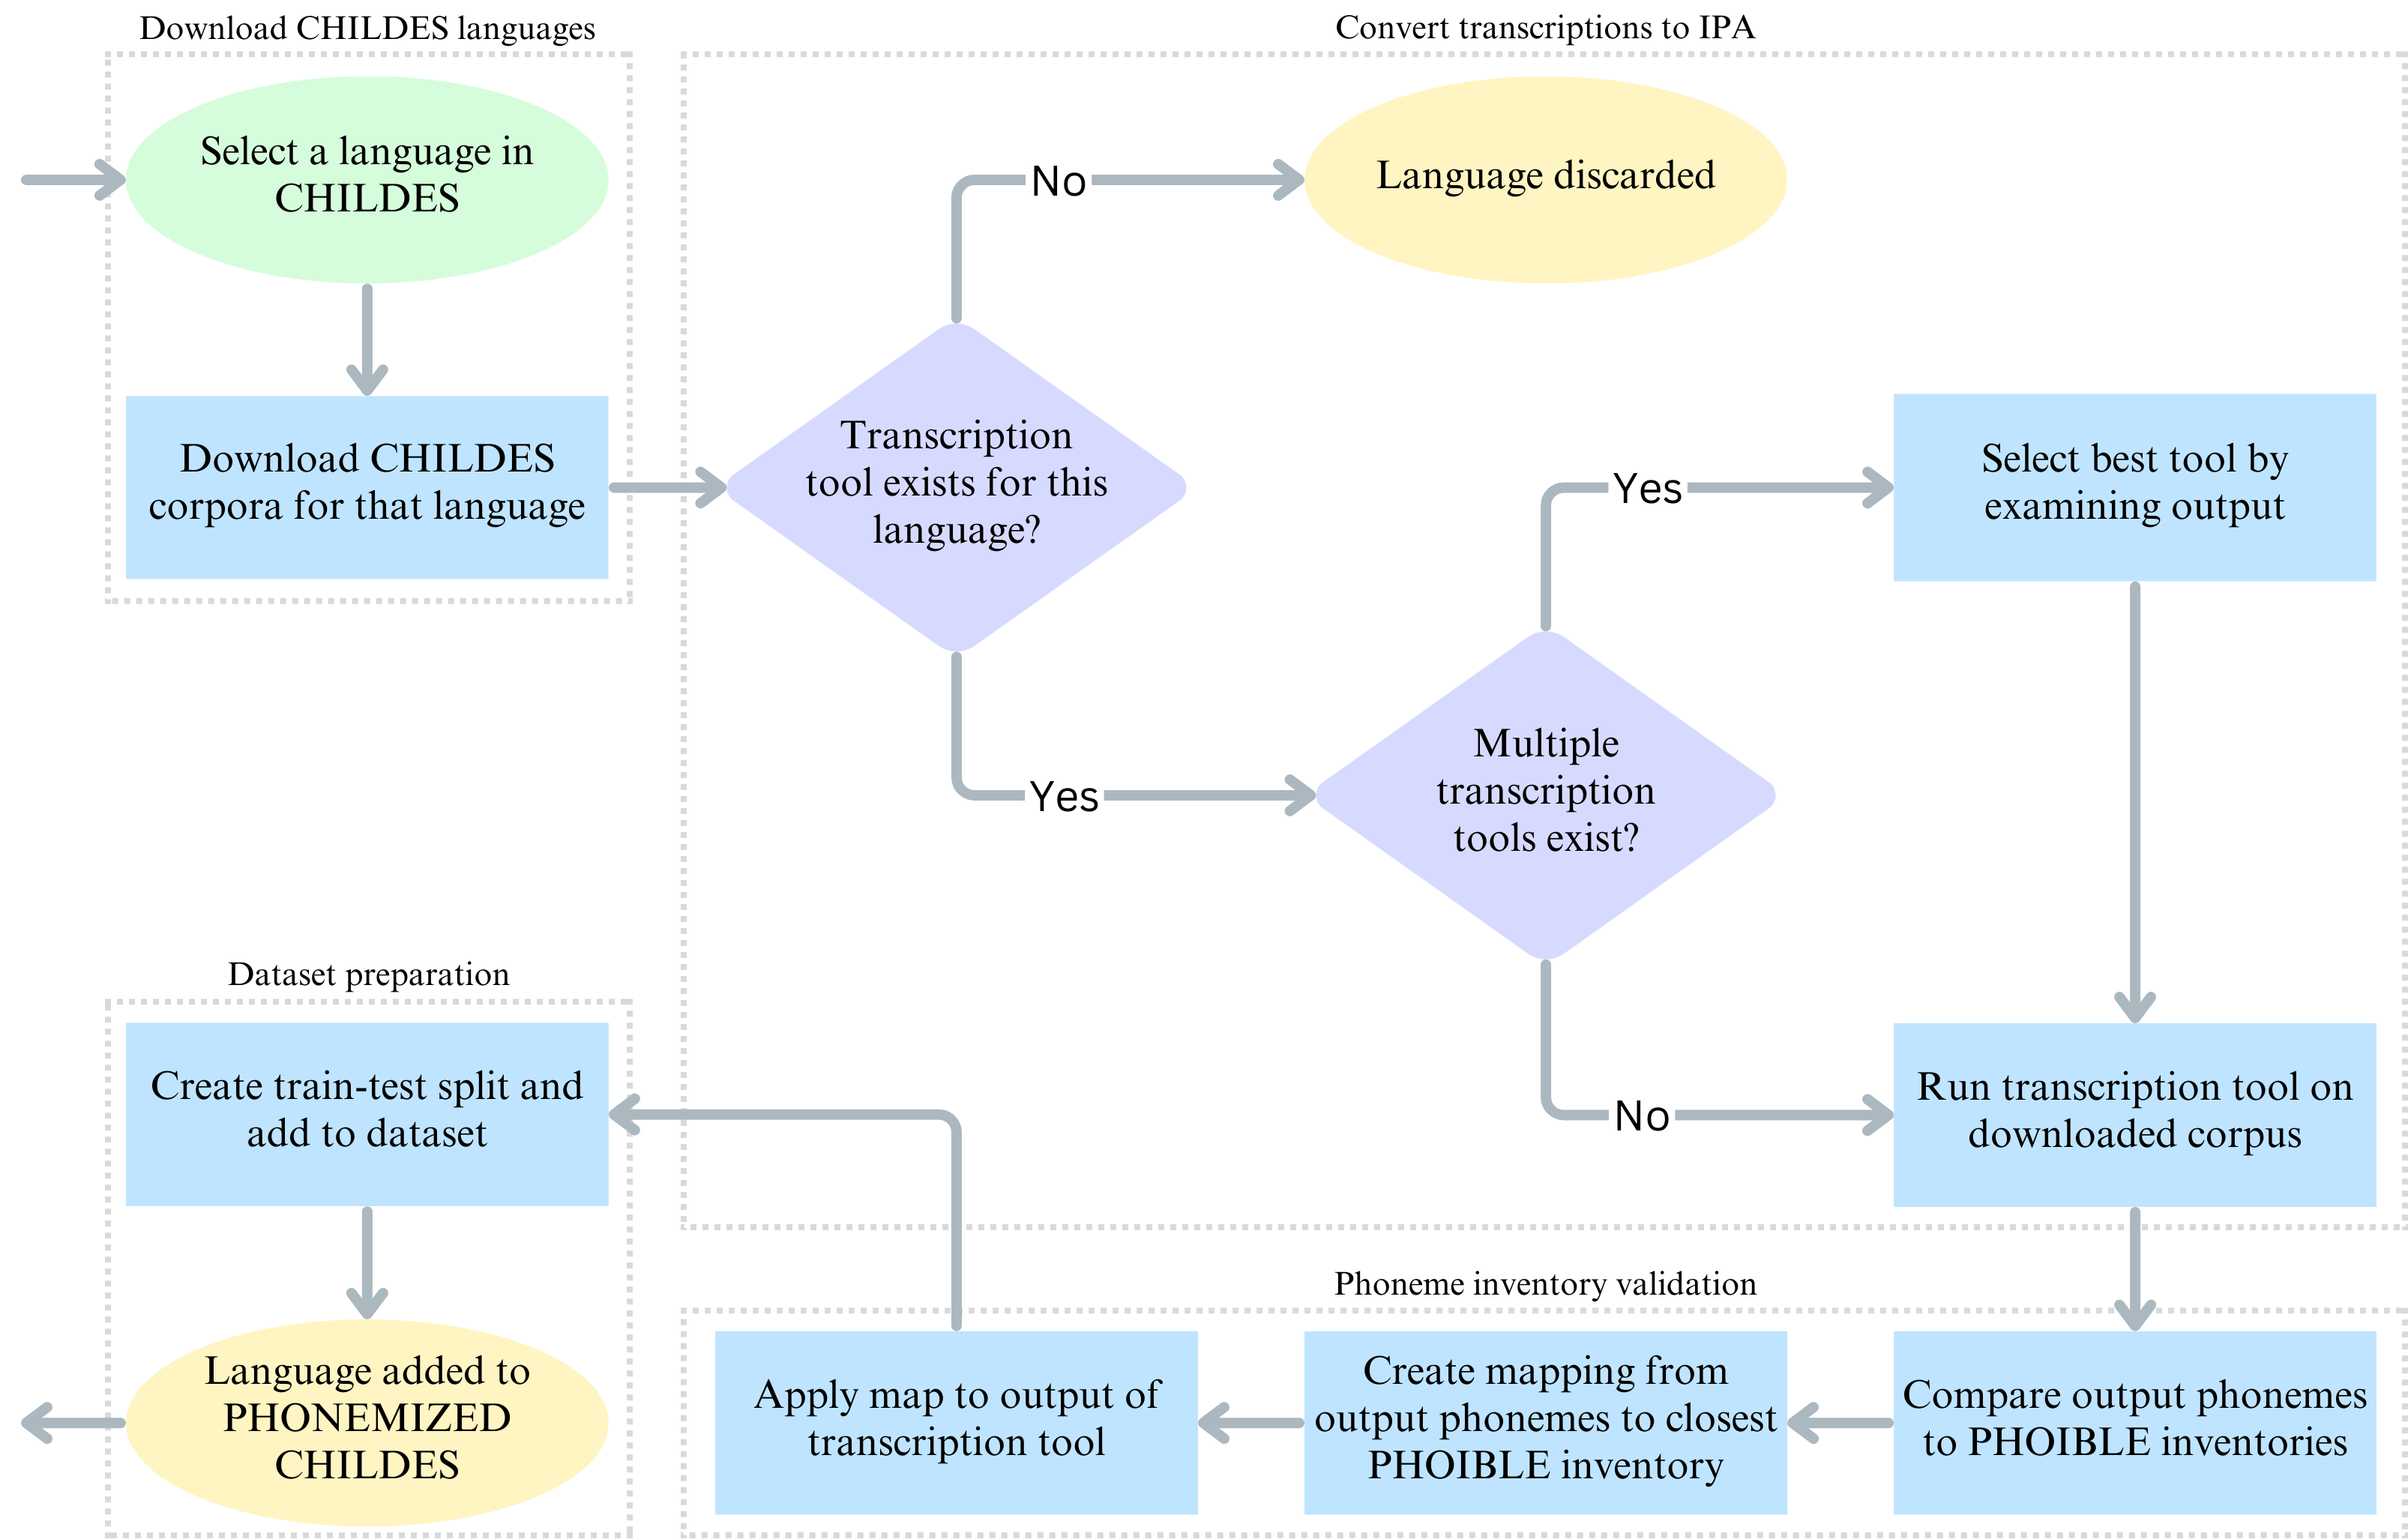
\includegraphics[width=0.9\linewidth]{Figures/13Dataset/data-prep.png}
    \caption{Data preparation pipeline for the \phonemizedchildes dataset.}
    \label{fig:dataset-phonemized-childes-prep}
\end{figure}

For each language hosted in CHILDES, I first use the \textbf{download} mode to individually download each corpus for that language that contain naturalistic child-directed utterances. I then assess whether \corpusphonemizer contains a backend and language code that supports that language. Unfortunately, this is not always the case. For instance, all Greek corpora in CHILDES are transcribed using a Latin script which is not supported by any of the backends in \corpusphonemizer. There are similar issues with Arabic, Hebrew, Thai, Georgian and Tamil.

If multiple backends support that language, I produce a transcription using each backend and carefully examine the output. The backend which produces a phonemic vocabulary which is closest to one of the phonemic inventories in \phoible is selected and is the backend for which I produce a folding map, as described in \cref{sec:dataset-folding}. I then run the \textbf{process} mode of CHILDES processor on all downloaded corpora for the language, using the selected backend and appropriate language code to phonemize the utterances (the folding map is automatically applied). This results in two CSV files for that language, a training set and a validation set containing 10,000 utterances.

Finally, I add the pair of CSV files to the \phonemizedchildes repository hosted on Huggingface. I then repeat this process for every language in CHILDES, resulting in 31 languages, as described in the next section. 

\subsection{Dataset overview}
\label{sec:dataset-phonemized-childes-overview}

The \phonemizedchildes dataset contains over seven million utterances of child-directed speech across 31 languages. Each language is available as a subset, with a `train' split containing the majority of the utterances downloaded from CHILDES and a `valid' split containing 10,000 utterances for validation purposes. An overview of each section is given in \cref{tab:dataset-phonemized-childes-sections}, detailing the corresponding CHILDES collection, the number of corpora downloaded, the backend and language code used with \corpusphonemizer to convert the corpora to phonemes and a numerical overview of the size of each section. Note that English is split into two sections to mirror the split present in CHILDES and Portuguese is split into two sections due to the phonological differences between Brazilian and Portugal Portuguese, the availability of language codes to phonemize the two, and the fact that the corpora are distinct within CHILDES.

\begin{table}[t]
    \centering
    \scriptsize
    \begin{tabular}{llllcccc}
        \toprule
        \textbf{Language} & \textbf{CHILDES Collection} & \textbf{Backend} & \textbf{Lang Code} & \textbf{Speakers} & \textbf{Utterances} & \textbf{Words} & \textbf{Phonemes} \\
        \midrule
        English (US)  & Eng-NA (44) & phonemizer & en-us & 2,692  & 1,645,797  & 7,096,724  & 22,107,530 \\
        English (UK)  & Eng-NA (14) & phonemizer & en-gb & 588  & 1,246,211  & 5,170,088  & 15,710,282 \\
        German  & German (10) & epitran & deu-Latn & 628  & 860,297  & 4,827,996  & 14,821,812 \\
        Japanese  & Japanese (9) & phonemizer & japanese & 329  & 557,215  & 1,773,816  & 7,100,307 \\
        Indonesian  & EastAsian/Indonesian (1) & epitran & ind-Latn & 389  & 534,525  & 2,122,372  & 6,369,459 \\
        French  & French (11) & phonemizer & fr-fr & 722  & 432,133  & 1,995,063  & 5,510,523 \\
        Spanish  & Spanish (18) & epitran & spa-Latn & 562  & 288,372  & 1,567,124  & 4,553,108 \\
        Mandarin  & Chinese/Mandarin (15) & pinyin\_to\_ipa & mandarin & 883  & 324,071  & 1,506,475  & 4,397,546 \\
        Dutch  & DutchAfricaans/Dutch (4) & phonemizer & nl & 78  & 261,938  & 1,106,865  & 3,585,608 \\
        Serbian  & Slavic/Serbian (1) & epitran & srp-Latn & 199  & 226,266  & 1,054,074  & 3,067,398 \\
        Estonian  & Other/Estonian (9) & phonemizer & et & 118  & 103,343  & 544,680  & 2,226,518 \\
        Cantonese  & Chinese/Cantonese (2) & epitran & yue-Latn & 81  & 147,673  & 651,392  & 1,824,730 \\
        Polish  & Slavic/Polish (2) & phonemizer & pl & 466  & 80,412  & 381,940  & 1,599,152 \\
        Swedish  & Scandinavian/Swedish (3) & phonemizer & sv & 32  & 85,299  & 396,800  & 1,242,615 \\
        Portuguese (Pt)  & Romance/Portuguese (3) & phonemizer & pt & 33  & 81,444  & 368,032  & 1,117,010 \\
        Korean  & EastAsian/Korean (3) & phonemizer & ko & 95  & 66,576  & 201,078  & 1,074,044 \\
        Italian  & Romance/Italian (5) & phonemizer & it & 92  & 57,542  & 264,479  & 996,701 \\
        Catalan  & Romance/Catalan (5) & phonemizer & ca & 159  & 56,588  & 248,999  & 839,462 \\
        Croatian  & Slavic/Croatian (1) & phonemizer & hr & 51  & 55,288  & 214,949  & 805,530 \\
        Welsh  & Celtic/Welsh (2) & phonemizer & cy & 65  & 55,871  & 269,295  & 785,569 \\
        Icelandic  & Scandinavian/Icelandic (2) & phonemizer & is & 15  & 50,657  & 197,519  & 751,804 \\
        Danish  & Scandinavian/Danish (1) & phonemizer & da & 25  & 48,976  & 192,527  & 579,972 \\
        Norwegian  & Scandinavian/Norwegian (2) & phonemizer & nb & 27  & 35,547  & 175,952  & 559,340 \\
        Basque  & Other/Basque (2) & phonemizer & eu & 150  & 36,614  & 135,866  & 565,633 \\
        Hungarian  & Other/Hungarian (3) & epitran & hun-Latn & 65  & 36,272  & 147,334  & 588,934 \\
        Romanian  & Romance/Romanian (2) & phonemizer & ro & 21  & 31,550  & 110,067  & 380,577 \\
        Portuguese (Br)  & Romance/Portuguese (2) & phonemizer & pt-br & 163  & 12,471  & 91,484  & 303,998 \\
        Irish  & Celtic/Irish (2) & phonemizer & ga & 20  & 18,256  & 88,388  & 278,558 \\
        Turkish  & Other/Turkish (2) & phonemizer & tr & 35  & 14,487  & 43,823  & 230,737 \\
        Quechua  & Other/Quechua (2) & phonemizer & qu & 7  & 13,425  & 33,102  & 204,692 \\
        Farsi  & Other/Farsi (2) & phonemizer & fa-latn & 23  & 13,467  & 28,080  & 115,089 \\
        \bottomrule
    \end{tabular}
    \caption{A breakdown of each language available as a subset of \phonemizedchildes. The bracketed number in the \textbf{CHILDES Collection column} refers to the number of corpora downloaded from that collection. The \textbf{Backend} and \textbf{Lang Code} columns refer to the \corpusphonemizer configuration used to convert utterances for that language to phonemes. The \textbf{Speakers} column refers to the number of unique speakers in each subset. The final three columns describe the size of the subset at three levels of analysis.}
    \label{tab:dataset-phonemized-childes-sections}
\end{table}
\todo[inline]{Possibly need to add the Phoible phoneme inventory information to this table, although perhaps that can be in the appendix.}

The dataset is hosted on Huggingface and can be loaded using Huggingface's \texttt{datasets} library \citep{lhoest-etal-2021-datasets} or downloaded directly. The dataset is stored as CSV files with one utterance per row, maintaining the structure of the CHILDES database. Both the original orthographic utterances and phonemized utterances are available, as well as many features imported from CHILDES, such as target child age, morpheme count, part of speech information, and the IDs of each utterance, transcript, corpus and collection. Within each section, the transcripts are sorted by target child age, to age-ordered curriculum learning experiments such as in the work of \citet{huebner-etal-2021-babyberta}.

\subsection{Corpus analysis}
\label{sec:dataset-phonemized-childes-analysis}

There is considerable variation in size between each subset in \phonemizedchildes. The largest subset is \textbf{English (US)} with over 1.6 million utterances and the smallest section is \textbf{Farsi} with only 13 thousand utterances. As these subsets reflect the number of utterances available for each language in CHILDES, which in turn come from individual corpora collected from acquisition research into that language, these differences give a sense of which languages are understudied in the field of acquisition, and the extent to which English dominates\todo{rewrite}. In this section, I compare each language in \phonemizedchildes according to their information-theoretic properties,   

\rough{A broad overview of the phonemic properties of each language within the corpus. A few experiments to justify why we use phonemes instead of letters, trying to highlight that phonemes are a more consistent representation for our purposes. Experiments include:
\begin{itemize}
    \item Information theoretic properties (Zipf's law, Heap's law, ratios, information rate, n-gram perplexities)
    \item Comparing phoneme properties to character properties (hypothesis: information rate more consistent across langugages when looking at phonemes rather than characters)
    \item Child vs adult speech (extract child utterances in CHILDES and compare MLU, word length etc)
    \item Child-directed vs adult-directed speech (compare CHILDES to BNC)
    \item Phoneme clustering (could possibly be moved to chapter 5 - segmentation): looking at phoneme clusters, possibly vowel harmony and other signals for segmentation.
    \item Child errors (could be moved to chapter 6 - past tense formation): looking at errors that children produce.
\end{itemize}
}

\section{Limitations of Automated Phonemization[?]}

\rough{Optional section to describe the Phonemized BNC and experiments where I compare the automated phonemization to the human transcriptions included in Audio BNC. Can serve as an in-depth exploration of the limitations of this approach.}

\todo[inline]{If this section is included, remove limitations section from \cref{sec:dataset-limitations}.}

\section{Summary}

\rough{We now have suitable corpora for training language models on phonemes across many languages, and for evaluating certain properties of languages. Etc.}